% Template for a Thesis
%
% 4-translation.tex
%
% Translation

\chapter{Translation}\label{ch:translation}

\section{Statistical machine translation (SMT)}

SMT is a machine translation approach where translations are generated based on statistical models, whose parameters are derived from the analysis of bilingual text corpora. It can be done with rule-based approaches in a supervised way, or example-based approach, unsupervised.

Pioneered at IBM in the early 1990s, the basis of SMT is information theory, a mathematical theory proposed by Claude Shannon in 1948 to find fundamental limits on signal processing and data compression. A documenti s translated according to the probabilistic distribution P(e|s) that a word \emph{e} in the target language (for example English) is the translation of a word \emph{s} in the source language (for example, Spanish).

\begin{itemize}
	\item P(e|s)
	\item Suppose that s = de nada
	\item P(you're welcome | de nada) = 0.45
	\item P(nothing | de nada) = 0.13
	\item P(water | de nada)= 0.00001
\end{itemize}

Typically, first a translation model translates the source language into a broken version of the target language, using an algorithm such as the expectation-maximization algorithm. Afterwards, a language model in the target language makes the broken language look more like it would if native speakers would use it. A good language model will for example assign a higher probability to the sentence "the house is small" than to "small the is house". An example of a translation system from Spanish to English can be seen below:

\begin{figure}[!ht]
    \centering
    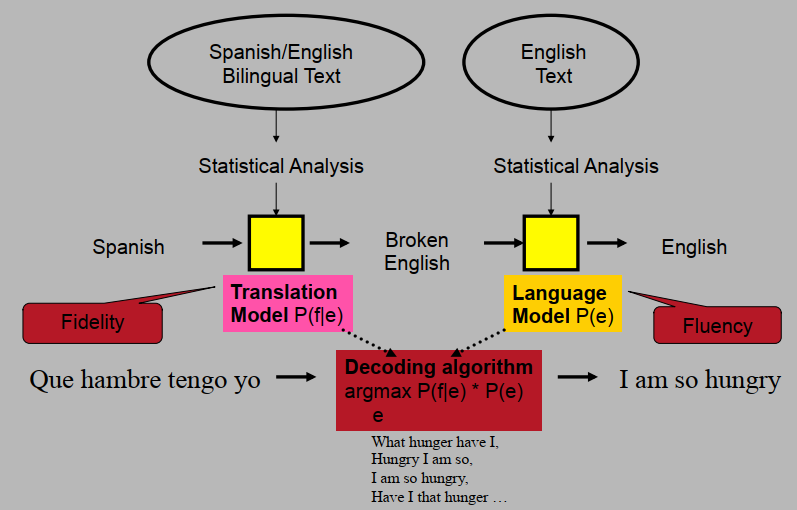
\includegraphics[width=10cm]{figures/smt.png}
    \caption{Example of Spanish-English SMT system.}
\end{figure}

The translation model in the first step needs to know which words to align in a source-target sentence pair. More in the next section.

\section{Word alignments}

Word alignment between two texts is the NLP task of identifying translation relationships among the words in a parallel text, resulting in a graph between the two sides of the texts, with an arc between two words if they are translations of one another. See the following example:

\begin{figure}[!ht]
    \centering
    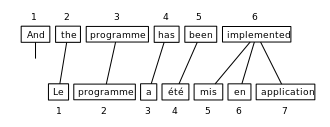
\includegraphics[width=10cm]{figures/word_align.png}
    \caption{Word alignments between an English and French sentence.}
\end{figure}

Alternatively, the alignments can also be displayed in a matrix:

\begin{figure}[!ht]
    \centering
    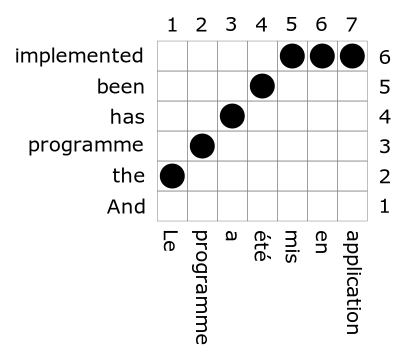
\includegraphics[width=8cm]{figures/word_align_matrix.png}
    \caption{Word alignments between an English and French sentence in matrix form.}
\end{figure}

In this example, the alignments aren't 1-on-1. Some words have a direct alignment, such as \emph{the}-\emph{le}, \emph{programme}-\emph{programme} and so on, but some words don't have an alignment (\emph{And}), and some have multiple alignments, in this case one-to-many: \emph{inmplemented}-\emph{mis en application}. There can also be many-to-one and many-to-many alignments.

Word alignment is an important task for most methods of statistical machine translation, since the parameters of these methods are usually estimated by observing word-aligned texts~\cite{brown1993mathematics}, and automatic word alignment is typically done by choosing that alignment which best fits a statistical machine translation model. A popular algorithm to find word alignments is the \emph{expectation-maximization algorithm}~\cite{och1999improved}

This approach is an example of unsupervised learning, meaning that the system has no knowledge of the kind of output desired, but tries to find values for the unobserved model and alignments which best explain the observed parallel text. In some cases, a small number of manually aligned sentences, in a way to explore supervised learning.~\cite{varga2007parallel} These models are usually able to more easily take advantage of combining many features within the data, such as context, syntactic structure, part-of-speech or translation lexicon information, which are difficult to integrate into the unsupervised models generally used.

For training, historically IBM models have been used.~\cite{koehn2009statistical} These models are used in statistical machine translation to train a) a translation model, and b) an alignment model. They make use of the expectation-maximization algorithm explained above: in the expectation step, the translation probabilities within each sentence are computed; in the maximization step, these probabilities are accumulated to global translation probabilities.

\subsection{Fastalign algorithm}

Fastalign algorithm~\cite{dyer-etal-2013-simple}

is a simple log-linear reparametrization of IBM Model 2 that overcomes problems from both Model 1 and Model 2. Training this model is consistently ten times faster than Model 4.

An open-source implementation of the alignment model described in this paper is available in \href{http://github.com/clab/fast align}{Github}.

Fastalign is a variation of the lexical translation. Lexican translation works as follows: given a source sentence \emph{f} with length \emph{n}, first generate the length of the target sentence \emph{m}, where the target sentence is \emph{e}. Then generate an alignment vector of length \emph{m} that indicates which source word (or null token) each target word will be a translation of. Lastly, generate the \emph{m} output words, where each word in \emph{e} depends only on the word in \emph{f} it's aligned with.

Fastalign's modification is that the distribution over alignments is parametrized by a null alignment probability and a precision parameter, which controls how strongly the model favors alignment points close to the diagonal (if we use the word alignment matrix like in the example above).

The paper~\cite{dyer-etal-2013-simple} has more detailed information on training, inference and results.

\subsection{Eflomal algorithm}

https://github.com/robertostling/eflomal
https://content.sciendo.com/view/journals/pralin/106/1/article-p125.xml